\section{Problemática}

  Una problemática relevante en el uso de herramientas de inteligencia artificial (IA) en la educación es la preocupación por la ética en la resolución de problemas, además de la dependencia excesiva de estas tecnologías para el aprendizaje. La automatización de tareas y la generación de respuestas rápidas pueden limitar el desarrollo de habilidades críticas y creativas en los estudiantes, afectando su capacidad para resolver problemas de manera independiente y analítica.

  Así mismo el uso indiscriminado de la información brindada por estas herramientas aún cuando explicitamente se menciona que puede ofrecer resultados erroneos o no confiables, puede llevar a una disminución en la capacidad de pensamiento crítico de los estudiantes, lo cual puede afectar su rendimiento académico.
  
  \begin{figure}[ht]
    \centering
    \begin{tikzpicture}
        \begin{axis}[
            width=0.8\textwidth, % Ancho del gráfico
            height=0.5\textheight, % Altura del gráfico
            xlabel={Año}, % Etiqueta del eje X
            ylabel={Usuarios (millones)}, % Etiqueta del eje Y
            xtick={2020, 2021, 2022, 2023, 2024}, % Ticks del eje X
            ytick={0, 50, 100, 150, 200}, % Ticks del eje Y
            ymin=0, % Límite inferior del eje Y
            ymax=200, % Límite superior del eje Y
            bar width=0.5cm, % Ancho de las barras
            enlarge x limits=0.15, % Ampliar límites en el eje X
            ylabel near ticks, % Posicionar la etiqueta del eje Y cerca de los ticks
            xlabel near ticks, % Posicionar la etiqueta del eje X cerca de los ticks
            grid=major, % Mostrar la cuadrícula
            title={Usuarios de ChatGPT por Año}, % Título del gráfico
            xticklabel style={align=center}, % Alinear los ticks del eje X
        ]
            \addplot[
                ybar,
                color=blue % Color de las barras
            ] 
            coordinates {(2020, 0.1) (2021, 0.5) (2022, 5) (2023, 100) (2024, 200)};
        \end{axis}
    \end{tikzpicture}
    \caption{Crecimiento de usuarios de ChatGPT desde su lanzamiento.}
    \label{fig:usuarios_chatgpt}
  \end{figure}
    
  Gráficos que describe la recepción y uso de ChatGPT en la población mundial desde su implementación. Puede observarse un crecimiento exponencial en el número de usuarios, lo que sugiere una mayor adopción de esta tecnología en diversos ámbitos, incluyendo la educación. Este aumento en la popularidad de ChatGPT plantea la necesidad de evaluar su impacto en el aprendizaje y desarrollo de habilidades de los estudiantes, así como de identificar posibles riesgos y desafíos asociados con su uso.

